\section{Preliminaries}\label{sec:pre}

The goal of the IPA algorithm is to find the optimal transmission power of any secondary transmitter. The optimal transmission power maximizes the transmission range of the secondary transmitter while causing no interference to any primary users. To find this power, a secondary transmitter needs knowledge of the radio propagation conditions and the presence of any primary transmitters. 
\subsection{Local power variance}

Radio propagation is typically modeled by a model consisting of three components: a distance dependent path loss trend, shadowing and fast fading. Shadow losses cause the received signal strength (RSS) to vary slowly in time and space around the distance dependent trend. Fast fading originates from multipath effects and causes the RSS to vary on a small scale \cite{bookPathlossModel}. Pollin, Adams and Bahai deduce from experiments that propagation conditions are difficult to model globally\footnote{In the measurement campaign of Pollin, Adams and Bahai \cite{sofie} the RSS from an 802.11 antenna on top of Cory Hall at UC Berkeley is measured in the area. They make three observations from the measurements. First, there is no obvious relationship between the RSS and the distance between the transmitter and the receiver. Second, the measurements show that shadowing is an anisotropic effect. Last, fast fading causes the RSS measurements to be noisy.}\cite{sofie}. Therefore, the IPA algorithm does not rely on a global propagation model but uses only local RSS measurements.

\subsection{Distance to contour flooding}
To detect the primary users and compute the distance between the transmission range of a primary user and the secondary user, no expensive sensing techniques are used. Instead, a more cost efficient distance-to-contour (DTC) flooding algorithm is used. This algorithm uses a back-off timer to decrease the number of forwarded messages with respect to regular flooding \cite{dtc}. With the DTC flooding algorithm, the number of forwarded messages is slightly larger than $n$, with $n$ being the number of users in the network. In this paper we develop an alternative distance-to-contour flooding algorithm which decreases the number of forwarded messages. This adapted flooding algorithm, DTC2, is based on the polygon tiling algorithm proposed by Hur et. al. \cite{dtc2}.

%%%%%%%%%%%%%%%%%%%%%%%%%%%%%%%%%%%%%%%%%%%%%%%%%%%%%%%%%%%%%%%%%%%%%%%%%%%%%%%%%%%%%%%%%%%%

\section{Iterative power adjustment algorithm}\label{sec:ipa}

\subsection{Overview}

We give an overview of the IPA algorithm in a situation with one primary and one secondary transmitter. However, the algorithm is also applicable in scenarios with multiple primary transmitters.
When the RSS of a user is used in the algorithm, an estimate $\hat{RSS}$ is computed with a MLS algorithm to average out the noise due to fast fading. This procedure is discussed in section \ref{sec:power est}.

First, receivers of the primary transmitters compute their $\hat{RSS}$ to find the users that define the interference threshold contour of the primary transmitter. Next, every user in the network is informed about his distance to the contour by means of the DTC flooding algorithm. DTC is discussed in section \ref{sec:dtc1}. Based on the distance to the contour of the primary transmitter and a worst case path loss model, a secondary transmitter can now make a first estimate of its transmission power. This initial estimate can iteratively be made more accurate based on information about the propagation conditions between the secondary and primary transmitter. First, the new contour-contour distance is taken into account. Second, the path loss between the contour of the secondary and primary transmitter is estimated at the user that is closest to the primary transmitter and still within the transmission range of the secondary transmitter. We discuss the iterative adaptation of the transmission power in section \ref{sec:pathloss est}.

\subsection{Local received power estimation} \label{sec:power est}

Reliable RSS estimates are needed for two reasons: To determine the interference threshold contours and to make accurate path loss estimations. The individual RSS measurements are noisy due to fast fading. In order to average out this noise, a MLS algorithm is used. This has the advantage that it does not rely on a global path loss model.

The MLS algorithm does not only take into account the RSS measurement of the user where the estimate is computed but also the measurements from the neighboring users. The size of the neighborhood is defined by a spatial weighting function (also called \textit{kernel function}). Assume we want to determine the $\hat{RSS}$ of user $N$ at position $x_N$. We search the coefficients $\vec{a}$ of a polynomial $\vec{p}$ by minimizing the weighted least squares function from equation \ref{eq:wls}. Polynomial $\vec{p}$ approximates the local RSS variations in the environment. To find $\vec{a}$, the local received power $RSS_N$ of user $N$ is taken into account together with the local received power $RSS_i$ of the neighbors of $N$, with $i=1..\#$Neighbors :
\begin{equation} \label{eq:wls}
\hat{\vec{a}}_N = \arg \min_a \sum_i w_{Ni}(\vec{a}^T \vec{p}(\vec{x}_i)-\vec{RSS_i})^2 \nonumber
\end{equation}
The local RSS measurements are weighted by $w_{Nj}$ according to the distance from user $N$, as demonstrated here:
\begin{equation} \label{eq:wij}
w_{Ni} = \begin{cases} 
(1-r_{Ni}^2)^3 &  \text{, if $r_{Ni} \leq 1$} \nonumber \\ 
0 & \text{, otherwise}
\end{cases}
\end{equation}
$r_{Ni}$ is the normalized distance between user $N$ and $i$. The distance is normalized by the kernel width $h$ as follows: $r_{Ni}=\frac{\begin{Vmatrix}\vec{x}_N-\vec{x}_i\end{Vmatrix}}{h}$.
From the coefficients $\hat{\vec{a}}_N$ we can compute $\hat{RSS}_N$ as:
\begin{equation}
\hat{RSS}_N = \hat{\vec{a}}^T_N \cdot \vec{p}(\vec{x}_N) \nonumber
\end{equation}

The MLS algorithm has two parameters: kernel width $h$ and the polynomial order of $\vec{p}$. These parameters depend on the noise power and can be optimized with respect to the average squared error on $\hat{RSS}$. This is demonstrated in the work of Pollin, Adams and Bahai \cite{sofie}. 

\subsection{Distance to contour flooding} \label{sec:dtc1}

An efficient flooding algorithm based on the algorithm proposed by Ye, Chen, Lu and Zhang \cite{dtc} is used to signal the presence of primary transmitters. The goal of the distance-to-contour flooding algorithm is to inform every user in the network about his distance to the contour of the primary user. A potential secondary transmitter can then determine the position of the wireless user within its transmission range that is closest to the contour of the primary user. In the next step of the IPA algorithm the path loss estimate of this closest secondary user is used to improve the estimate of the optimal transmission power of the secondary transmitter.

The centralized version of the DTC algorithm uses a priority queue to keep track of all information. Consider a scenario with transmitter P and $n$ wireless users. All users that receive P with a RSS larger than the interference contour threshold, $RSS_{th}$, are within the transmission range of P and are called \textit{internal} users. The \textit{footpoint} $f_i$ of a user $i$ with respect to P is defined as the internal user of P that is closest to $i$. The goal of the distance-to-contour algorithm is to inform all users about their footpoint $f$ and the distance $d$ to this footpoint.


\begin{enumerate}
\item During initialization all internal users of P are added to a priority queue. The footpoint of an internal user is the position of the user himself, $f_i = x_i$, and thus $d(i,f_i) = 0$. For all other users $d = \infty$.
\item The user with the smallest distance, user $N$, is taken from the queue. If more users share this smallest distance, one is randomly selected
\item User $N$ now informs his one-hop neighbors about his footpoint $f_N=x_A$. Based on this information the neighbors of $N$ update their footpoint and distance as follows: consider user $M$ which is a neighbor of $N$. The footpoint of $M$ is $f_M=x_B$ with $d(x_M,x_B)$. There are two possibilities:
\begin{enumerate}
 \item If $d(x_M,x_A) < d(x_M,x_B)$ then \\	
	$f_M \leftarrow x_A$ and $d(M,f_M) \leftarrow d(x_M,x_A)$ 
	, and $M$ is added to the queue.
 \item If $d(x_M,x_A) \geq d(x_M,x_B)$ then $f_M$ does not change and $M$ is not added to the queue.
\end{enumerate} 
 
\item When all the neighbors of $N$ are updated, $N$ is removed from the queue. The next user is now taken from the queue and all his neighbors are updated.
\item The process is repeated until the queue is empty
\end{enumerate}


To minimize the number of forwarding messages in the distance-to-contour flooding algorithm, the order in which users update their neighbors depends on their distance from P. In the centralized algorithm this is implemented by using a priority queue. In a practical scenario where users only communicate with their one-hop neighbors a priority queue cannot be used. The algorithm is made distributed by implementing the distance dependence with a back-off timer. 

Ideally, the time in which the network is updated equals $CW \cdot h$, with $h$ the communication range. The number of messages equals $n$, with $n$ the number of users in the network. In a practical scenario the update time and number of messages will be larger due to two reasons: 
 
\begin{itemize}
 \item Retransmissions are necessary because of collisions.
\item It is possible that a user starts updating his neighbors before he has obtained his closest footpoint. Wrong information is propagated to the neighbors and the user will have to update his neighbors a second time once he obtained his correct footpoint. We say the neighbors are \textit{misclassified}. This is illustrated in Fig.~\ref{fig:misclass}.
\end{itemize}

\begin{figure}
\centering
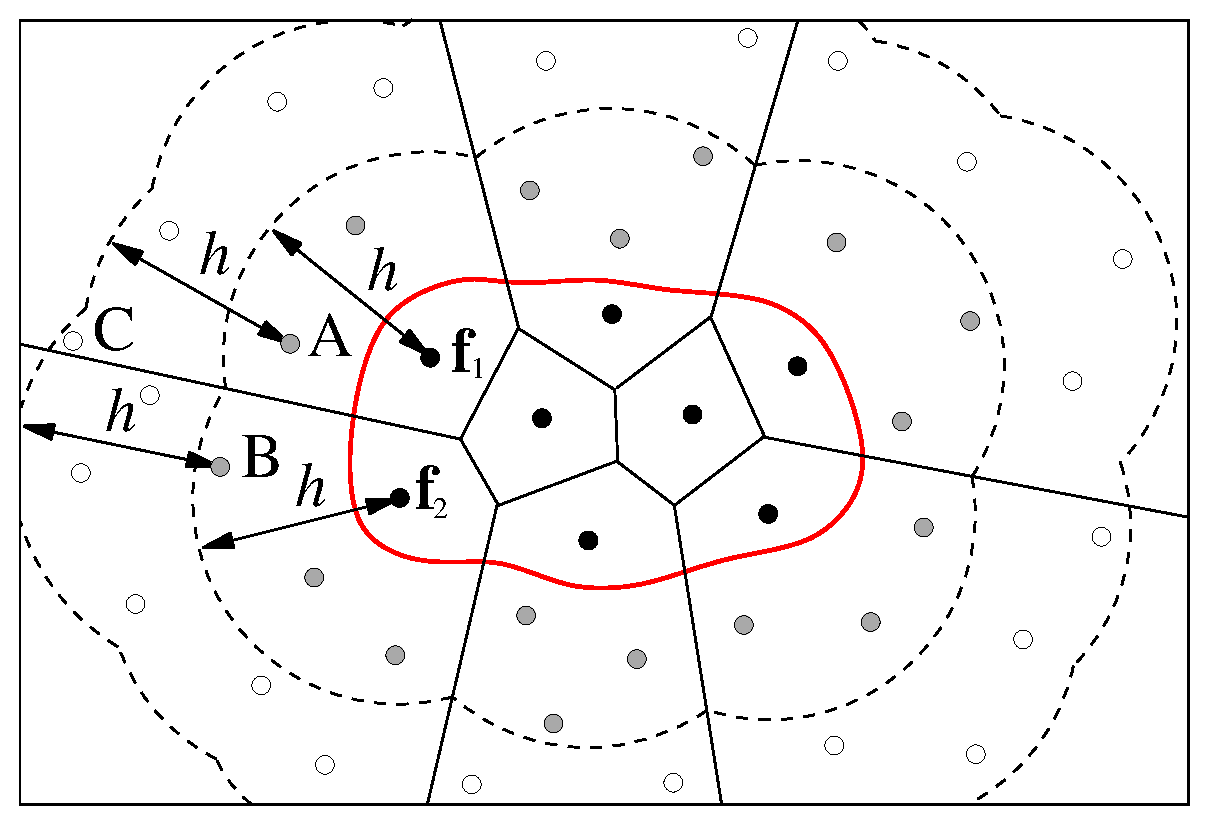
\includegraphics[scale=0.25]{figures/algorithm/proof2}
\caption{\label{fig:misclass}Users with the same footpoint are grouped together by a Voronoi Tiling. User C has footpoint $f_1$ and it lies in the transmission range of both users A and B. If the backoff timer of B goes off before the back-off timer of A, user C gets updated first by user B and it will incorrectly store $f_2$ as its footpoint. After user C is updated by user B, it starts a back-off timer to update its neighbors. However, when the back-off timer of user A goes off, C receives its correct footpoint $f_1$. If C has already updated its neighbors before it receives the update from A, user C will have to update its neighbors a second time. Figure from Pollin et.al. \cite{sofie} }
\end{figure}

\subsection{Path loss estimation} \label{sec:pathloss est}

When every user knows his distance to the contour of the primary transmitter P, a secondary transmitter S can estimate its optimal transmission power, $\hat{\textrm{power}}_S$, based on a local path loss estimate $\hat{PL}$ computed at the internal user of S that is closest to the primary contour, user $i_{cl}$. First, parameters $\alpha$ and $\beta$ of a path loss model are computed with a weighted least squares fit at $i_{cl}$. All the neighbors, $j$, within the kernel width $h$ around $i_{cl}$ are taken into account. This is shown in equation \ref{eq:fit}. Parameter $\alpha$ models the distance-dependent trend and $\beta$ consists of shadow and antenna losses. $d(S,j)$ is the distance between the transmitter S and a receiving user $j$. Next, the power of S is computed as the maximal interference power plus the estimated path loss between S and the contour of the primary transmitter. This is shown in equations \ref{eq:pow1} and \ref{eq:pow2}.
\begin{align}
&\hat{\alpha}_i,\hat{\beta}_i = \label{eq:fit} \\ \nonumber 
&\arg\min_{\alpha,\beta}\sum_j w_{ij}(\alpha10\log_{10} d(S,j)+\beta-\textrm{PL}_j)^2 \\
&\hat{\textrm{PL}}(S,f_{i_{cl}})=\hat{\alpha}10\log_{10}d(S,f_{i_{cl}})+\hat{\beta} \label{eq:pow1} \\
&\hat{\textrm{power}}_S=RSS_{th}+\hat{\textrm{PL}}(S,f_{i_{cl}}) \label{eq:pow2}
\end{align}

Note that it is hypothesized that the local path loss estimation at $i_{cl}$ gives information about the long range path loss between the primary and secondary transmitter. However, extrapolation over a long range and the presence of outliers can invalidate this hypothesis. We investigated a number of more complex approaches to solve this problem but they did not lead to a useful result. Further investigation is needed.

\subsection{Path loss model}

The IPA algorithm is tested in a simulated two-dimensional environment. In this section we present the path loss model used to simulate radio propagation conditions. The path loss $PL$ consists of four components which we discuss below: A distance dependent trend, antenna losses, shadowing and fast fading:
\begin{equation} \label{eq:plModel}
PL=10\alpha\log(d)+\gamma+L_S+X_{\sigma} \nonumber
\end{equation}
First, path loss increases exponentially with the distance $d$ from the transmitter. The rate of increase is modeled by parameter $\alpha$. Second, antenna losses are modeled by parameter $\gamma$. Third, shadow losses, $L_S$, are modeled by placing buildings in the scenario as explained in the work of Pollin, Adams and Bahai \cite{sofie}. Last, fast fading is modeled as Gaussian noise, $X_{\sigma}$, with variance $\sigma^2$. Pollin, Adams and Bahai showed that $\sigma^2=4$ is a realistic value for fast fading, thus this value is used in our simulations \cite{sofie}. However, the exact parameters of the path loss model are not important because the IPA algorithm only makes use of local path loss measurements.













